\chapter{Identification}
\section{Sputnik VAD}
% graphic of Sputnik construction
The Sputnik VAD is an axial-flow blood pump, developed in a cooperative project of the National Research University of Electronic Technology, OJSC Zelenograd Innovation-Technology Center of Medical Equipment, FSBI "Academician V.I. Shumakov Federal Research Center of Transplantology and Artificial Organs", Ministry of Health of Russian Federation, DONA-M LLC and BIOSOFT-M LLC in 2009. \cite{Sputnik1}
\\This device is used for left ventricular assistance in patients with acute heart failure. The therapeutic objective in implantation of a Sputnik VAD is bridging to transplantation. The VAD is able to pump up to 10 liters of blood per minute with a continuous flow profile. The implantable pump weighs about 200 g, has a length of 81 mm and a maximum diameter of $34\, mm$. It consists of a moving and a stationary part. The moving part, the impeller, which is a rotor with four blades, contains a permanent NdFeB-magnet which is actuated by a brushless DC motor. The rotor spins clockwise with speed values between $4000-10000\, rpm$. An overview of the pumps specification is presented in \tablename~ \ref{tab:sput1}
\begin{table}[h]
  \centering
  \begin{tabular}{c|c}
    \toprule
    Blood flow  & 0-10 L/min \\
    Rotational speed & 4000-10000 rpm \\
    Length & 81 mm \\
    Diameter & 34 mm \\
    Weight & 200 g \\
    \bottomrule
\end{tabular}
  \caption[Specifications of Sputnik VAD]{Specifications of Sputnik VAD}
  \label{tab:sput1}
\end{table}
The stator is located inside a titanium housing with a 16 mm diameter. The stationary part of the pump consists of a flow straightener with three stationary blades and a flow diffusor with three twisted blades. The flow straightener is located in front of the rotor and straightens the incoming blood flow into the rotor. Behind the rotor the blood is directed into the diffusor. %\cite{Sputnik1}
\figurename~ \ref{fig:sput_cross} depicts a cross-section of the Sputnik VAD and identifies its individual components.
The connection between the pump and the cardiovascular system is performed using in- and outflow cannulas, a felt ferule and vascular prosthesis which is sewed to the aorta. \cite{Sputnik1}
\begin{figure}[h]
  \centering
  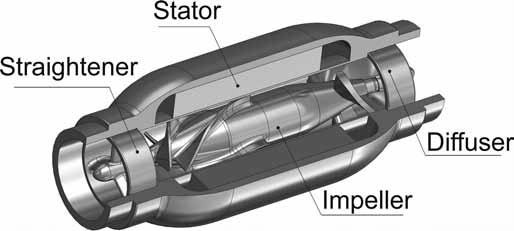
\includegraphics[width=0.6\textwidth]{images/sputnik_cross.png}
  \caption[Cross-section of Sputnik VAD \cite{Sputnik6}]{Cross-section of the Sputnik VAD \cite{Sputnik6}}
  \label{fig:sput_cross}
\end{figure}
The Sputnik VAD is powered using two lithium-ion batteries, fully loaded providing enough energy for up to eight hours of system support. The maximum charging time for the batteries is less than five hours. During this time the batteries can either be exchanged by another set of batteries or the system can be powered through connection to an AC network. A microprocessor-based driving unit is used to regulate the pump speed, manage the power supply and store parameter data. It is connected percutaneously to the pump with an up to 170 cm long and 5 cm wide lead. \cite{Sputnik1}

\section{Hardware in the Loop Test Bench}
%Aufbau

%Umbau

\section{System Identification}
%Vergleich Flüssigkeiten
%Vergleich Schlauchlängen
%Kennfeld
